\chapter{Introduction}
\label{Chapter1} 
%-------------------------------------------------------------------------------------
% Define some commands to keep the formatting separated from the content 
\newcommand{\keyword}[1]{\textbf{#1}}
\newcommand{\tabhead}[1]{\textbf{#1}}
\newcommand{\code}[1]{\texttt{#1}}
\newcommand{\file}[1]{\texttt{\bfseries#1}}
\newcommand{\option}[1]{\texttt{\itshape#1}}

%------------------------------------------------------------------------------------
Scientific visualization is now a critical tool in many domains, from medicine to engineering, allowing professionals to interpret complex data sets and extract meaningful insights (\cite{baines_2008}). One of the foundational techniques in scientific visualization is the representation of volume data, which often demands sophisticated methods to transform this data into visual models. Mesh generation, a technique that translates volumetric data into structured geometric models, is central to these methods (\cite{Wünsche_1997}). As the complexity of simulations and digital models escalates, there's an increasing demand for advanced and reliable mesh generation methods.

Isosurface extraction, a subset of mesh generation, has garnered significant attention due to its potential to represent intricate geometries from volume data (\cite{Lorensen_1987}). 
However, this technique has challenges, especially when dealing with Hermite data and the intricacies of conformal meshing. 
The selection of appropriate algorithms, the incorporation of ray tracing for enhanced visualization, and the overall optimization of these processes are all active research and exploration (\cite{Krüger_2003}).

This research endeavors to delve deep into these challenges, offering a comprehensive exploration of isosurface extraction techniques, their strengths, limitations, and potential areas of optimization. By understanding the nuances of these methods, this research aims to significantly contribute to the broader field of scientific visualization, providing insights and methodologies that further the academic understanding of the subject.

\section{Problem Description}

The rapid advancements in computational capabilities have led to the generation of increasingly complex and detailed volume data across various scientific domains. While this data holds invaluable insights, extracting meaningful information remains a significant challenge. The primary issue lies in transforming this volumetric data into structured geometric models that are both accurate and computationally efficient (\cite{Lorensen_1987}).

As a pivotal technique in mesh generation, isosurface extraction offers a promising solution to this challenge. However, its application is fraught with complications. The inherent nature of volume data, mainly when derived from sources like Hermite data, introduces complexities in achieving conformal meshing. This results in generated meshes that might not accurately represent the underlying data, potentially losing critical information (\cite{Wünsche_1997}).

Furthermore, while algorithms such as Dual Contouring and Dual Marching Cubes show promise, their practical implementation is not without issues. Challenges include the optimization of nested loop iterations, efficient data structuring, and the occasional inaccuracies in the Quadratic Error Function's implementation (\cite{Krüger_2003}).

Additionally, with the increasing demand for real-time applications in fields like gaming and interactive simulations, there's a pressing need for algorithms that generate accurate meshes and do so within the constraints of real-time rendering.

The core problem this research addresses is the development and optimization of isosurface extraction techniques that can efficiently and accurately transform complex volume data into meaningful geometric models suitable for a wide range of applications.

\section{Scope of Work}

The domain of scientific visualization, particularly in the context of volume data and mesh generation, is intricate and expansive. This research aims to comprehensively explore this domain, focusing on the challenges and intricacies of isosurface extraction and mesh generation. The following areas will be investigated:

\begin{itemize}
    \item \textbf{Mesh Generation and Volume Data:} A foundational exploration into the nature of volume data and its significance in mesh generation. The research will delve into the complexities introduced by Hermite data in the mesh generation process and elucidate the challenges and intricacies associated with conformal meshing using this data.
    
    \item \textbf{Ray Tracing and Mesh Visualization:} An exploration of the potential of ray tracing, especially with the Intel Embree API, for achieving realistic visualizations of generated meshes.
    
    \item \textbf{Comparative Analysis of Mesh Generation Methods:} A comparative analysis of various mesh generation methodologies, such as the Marching Cubes algorithm and its variations. The research will emphasize their unique strengths, challenges, and potential areas of improvement in generating accurate and detailed meshes.
    
    \item \textbf{Quadratic Error Function (QEF) in Mesh Algorithms:} An investigation of the QEF and its pivotal role in the Dual Contouring and Dual Marching Cubes algorithms for mesh generation. The study will dissect the methodology of QEF, understanding its significance and implications in the chosen algorithms.
\end{itemize}

\noindent By focusing on these areas, the research aims to offer a holistic understanding of mesh generation, challenges, methodologies, and significance in the broader domain of scientific visualization.


\section{Research Objective}

The primary objectives of this research are:
\begin{itemize}
    \item To understand the challenges and intricacies of conformal meshing through Hermite data.
    \item To explore and evaluate the performance of Dual Contouring and Dual Marching Cubes algorithms in isosurface extraction.
    \item To integrate and utilize the Intel Embree library for efficient ray tracing.
    \item To delve into the Quadratic Error Function's methodology and its significance in the chosen algorithms.
\end{itemize}

\section{Report Outline}
To provide a coherent and structured presentation of the methodologies and frameworks utilized in this thesis and to align them with the overarching objectives of the research, the chapter arrangement is delineated as follows:

\begin{figure}[ht!]
    \centering
    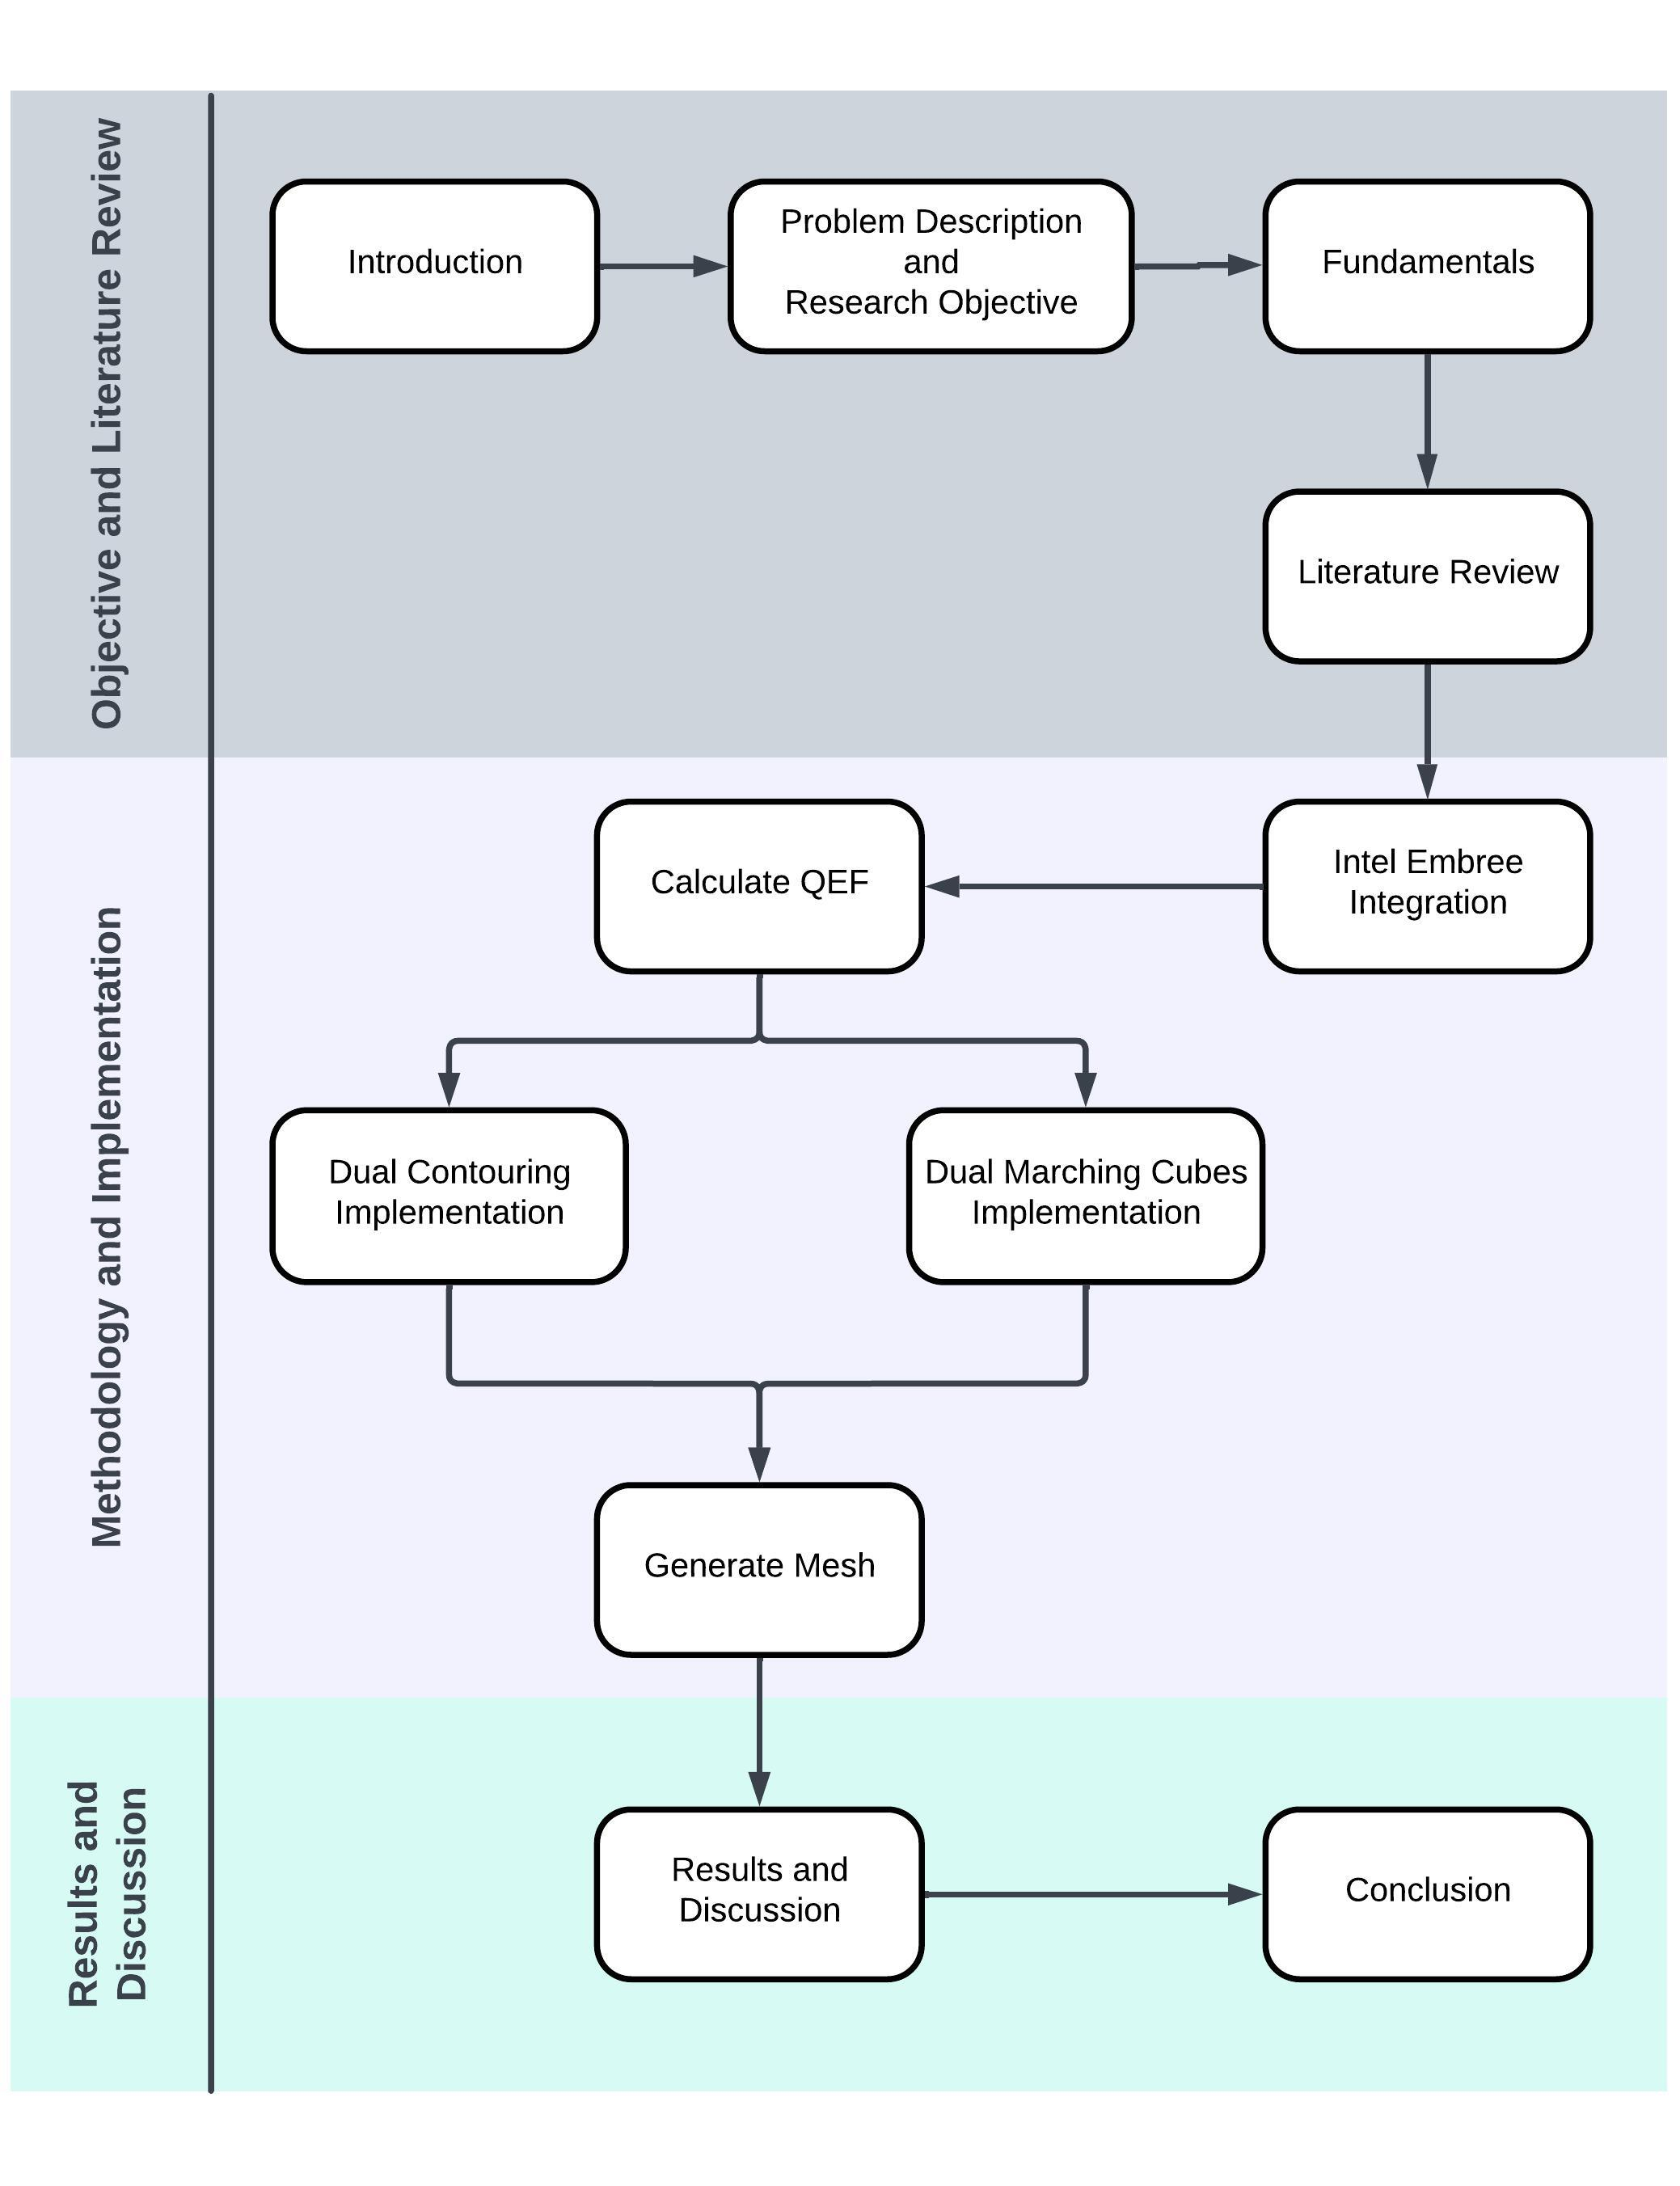
\includegraphics[width=0.9\textwidth]{Figures/Thesis-Report-Outline.jpeg}
    \decoRule
    \caption{Thesis report outline}
    \label{fig:Thesis-Report-Outline}
\end{figure}
\begin{itemize}
    \item \textbf{Chapter 1: Introduction} - This chapter introduces the problem domain, the scope of the research, and the objectives and provides an outline of the report.
    \item \textbf{Chapter 2: Fundamentals} - A deep dive into surface extraction, emphasizing the significance of meshes, challenges posed by Hermite data, and the importance of conformal meshing.
    \item \textbf{Chapter 3: Literature Review} - A comprehensive review of existing isosurface extraction methods, their strengths, and limitations.
    \item \textbf{Chapter 4: Embree API Integration} - Exploration of ray tracing using the Intel Embree library and foundational data structures supporting isosurface extraction algorithms.
    \item \textbf{Chapter 5: QEF Calculation using the Eigen Library} - A detailed examination of the Quadratic Error Function and its role in the Dual Contouring and Dual Marching Cubes algorithms.
    \item \textbf{Chapter 6: Implementation and Results} - Practical implementation of the Dual Contouring and Dual Marching Cubes algorithms, along with a discussion of their results.
    \item \textbf{Chapter 7: Conclusion and Future Work} - A summary of the research findings, their implications, and potential areas for future research.
\end{itemize}